% Created 2023-09-17 Sun 14:55
% Intended LaTeX compiler: pdflatex
\documentclass[11pt]{article}
\usepackage[utf8]{inputenc}
\usepackage[T1]{fontenc}
\usepackage{graphicx}
\usepackage{grffile}
\usepackage{longtable}
\usepackage{wrapfig}
\usepackage{rotating}
\usepackage[normalem]{ulem}
\usepackage{amsmath}
\usepackage{textcomp}
\usepackage{amssymb}
\usepackage{capt-of}
\usepackage{hyperref}
\author{Scott Jackson}
\date{\today}
\title{}
\hypersetup{
 pdfauthor={Scott Jackson},
 pdftitle={},
 pdfkeywords={},
 pdfsubject={},
 pdfcreator={Emacs 27.1 (Org mode 9.3)}, 
 pdflang={English}}
\begin{document}

\section*{This is a directory maze}
\label{sec:org2c20b25}

The point of this set of folders is to provide a bunch of nested directories to help students practice navigating directory structure.

\subsection*{Start Here}
\label{sec:org4c1fdc3}

The folders are numbered roughly from ``top'' to ``bottom'', and each has a simple text file with some simple contents, to help confirm where you are at any given time.

I recommend you use the \texttt{folder5} directory as a starting place, since it's roughly in the middle of the structure, and it gives you lots of options for where to go.

\subsection*{Map}
\label{sec:orge32499c}

Here's a schematic map to help:

\begin{center}
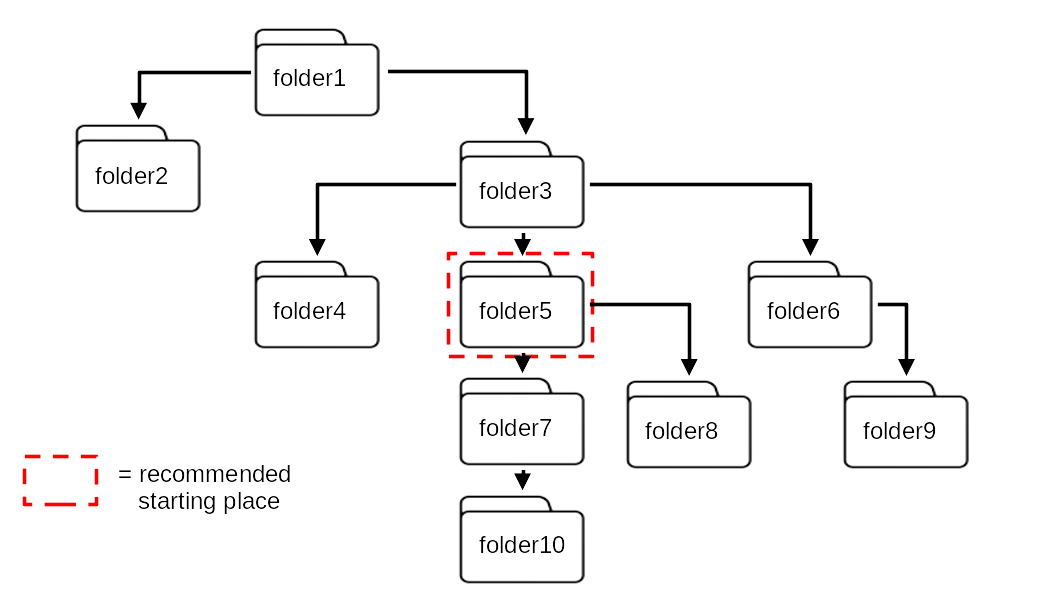
\includegraphics[width=.9\linewidth]{./folder_map.png}
\end{center}
\end{document}
